\documentclass{beamer}
\usepackage[utf8]{inputenc}

\usetheme{Madrid}
\usecolortheme{default}
\usepackage{amsmath,amssymb,amsfonts,amsthm}
\usepackage{mathtools}
\usepackage{txfonts}
\usepackage{tkz-euclide}
\usepackage{listings}
\usepackage{adjustbox}
\usepackage{tfrupee}
\usepackage{array}
\usepackage{gensymb}
\usepackage{tabularx}
\usepackage{gvv}
\usepackage{lmodern}
\usepackage{circuitikz}
\usepackage{tikz}
\lstset{literate={·}{{$\cdot$}}1 {λ}{{$\lambda$}}1 {→}{{$\to$}}1}
\usepackage{graphicx}

\setbeamertemplate{page number in head/foot}[totalframenumber]

\usepackage{tcolorbox}
\tcbuselibrary{minted,breakable,xparse,skins}



\definecolor{bg}{gray}{0.95}
\DeclareTCBListing{mintedbox}{O{}m!O{}}{%
  breakable=true,
  listing engine=minted,
  listing only,
  minted language=#2,
  minted style=default,
  minted options={%
    linenos,
    gobble=0,
    breaklines=true,
    breakafter=,,
    fontsize=\small,
    numbersep=8pt,
    #1},
  boxsep=0pt,
  left skip=0pt,
  right skip=0pt,
  left=25pt,
  right=0pt,
  top=3pt,
  bottom=3pt,
  arc=5pt,
  leftrule=0pt,
  rightrule=0pt,
  bottomrule=2pt,
  toprule=2pt,
  colback=bg,
  colframe=orange!70,
  enhanced,
  overlay={%
    \begin{tcbclipinterior}
    \fill[orange!20!white] (frame.south west) rectangle ([xshift=20pt]frame.north west);
    \end{tcbclipinterior}},
  #3,
}
\lstset{
    language=C,
    basicstyle=\ttfamily\small,
    keywordstyle=\color{blue},
    stringstyle=\color{orange},
    commentstyle=\color{green!60!black},
    numbers=left,
    numberstyle=\tiny\color{gray},
    breaklines=true,
    showstringspaces=false,
}

\title{5.8.11}
\date{September 14, 2025}
\author{Bhargav - EE25BTECH11013}

\begin{document}

\frame{\titlepage}
\begin{frame}{Question}
The coach of a cricket team buys $3$ bats and $6$ balls for \rupee 3900. Later, she buys
another bat and $3$ more balls of the same kind for \rupee 3300. Find the cost of a bat and
ball.

\end{frame}

\begin{frame}{Solution}
Let the cost of the bat, ball be \rupee x and \rupee y respectively.
\begin{align}
\myvec{3 & 6}\myvec{x \\ y} = 3900
\end{align}
\begin{align}
\myvec{1 & 3}\myvec{x \\ y} = 3300
\end{align}

These can be combined to give the matrix equation
\begin{align}
\myvec{3 & 6 \\ 1 & 3}\myvec{x \\ y} = \myvec{3900 \\ 3300}
\end{align}
\end{frame}

\begin{frame}{Solution}
This gives the augmented matrix
\begin{align}
\augvec{2}{1}{3 & 6 & 3900 \\ 1 & 3 & 3300} \xleftrightarrow{R_2 \leftarrow R_2 - \frac{1}{3}R_1} \augvec{2}{1}{3 & 6 & 3900 \\ 0 & 1 & 2000}
\end{align}

This gives the following values of x and y:
\begin{align}
\myvec{x \\ y} = \myvec{-2700 \\ 2000}
\end{align}

Thus, the cost of one ball is \rupee 2000 and the cost of one bat is - \rupee 2700
\end{frame}

\begin{frame}{Plot}
\begin{figure}[h!]
    \centering
    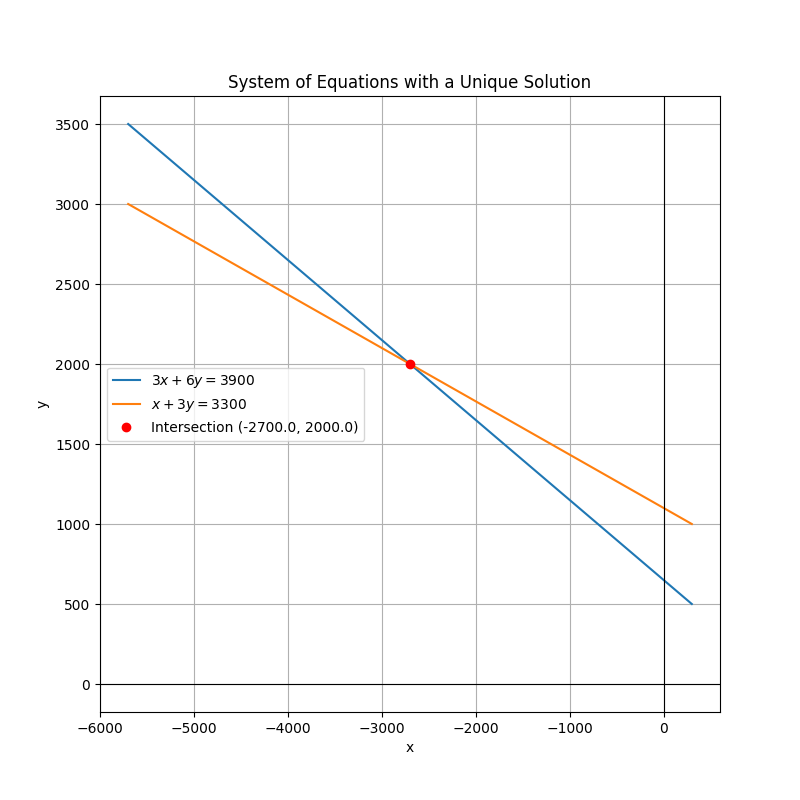
\includegraphics[height=0.5\textheight, keepaspectratio]{figs/Figure_1.png}
    \label{figure_1}
\end{figure}
\end{frame}

\begin{frame}[fragile]
    \frametitle{C Code}
    \begin{lstlisting}
#include <stdio.h>

int solve_2x2(double A[4], double b[2], double x[2]) {
    double det = A[0]*A[3] - A[1]*A[2]; 

    if (det == 0.0) {
        return -1; 
    }

    x[0] = (b[0]*A[3] - b[1]*A[1]) / det;
    x[1] = (A[0]*b[1] - A[2]*b[0]) / det;

    return 0; 
}


    \end{lstlisting}
\end{frame}



\begin{frame}[fragile]
    \frametitle{Python + C Code}
    \begin{lstlisting}
import numpy as np
import matplotlib.pyplot as plt
import ctypes
lib = ctypes.CDLL("./code.so")   
lib.solve_2x2.argtypes = [ctypes.POINTER(ctypes.c_double),
                          ctypes.POINTER(ctypes.c_double),
                          ctypes.POINTER(ctypes.c_double)]
lib.solve_2x2.restype = ctypes.c_int
A = np.array([[3, 6],
              [1, 3]], dtype=np.float64)
b = np.array([3900, 3300], dtype=np.float64)
x = np.zeros(2, dtype=np.float64)
status = lib.solve_2x2(A.ctypes.data_as(ctypes.POINTER(ctypes.c_double)),
                       b.ctypes.data_as(ctypes.POINTER(ctypes.c_double)),
                       x.ctypes.data_as(ctypes.POINTER(ctypes.c_double)))


    \end{lstlisting}
\end{frame}

\begin{frame}[fragile]
    \frametitle{Python + C Code}
    \begin{lstlisting}

if status == 0:
    x_sol, y_sol = x
    print(f"The system has a unique solution:")
    print(f"x = {x_sol}")
    print(f"y = {y_sol}")
    x_vals = np.linspace(x_sol - 3000, x_sol + 3000, 400)
    y1 = (3900 - 3 * x_vals) / 6
    y2 = (3300 - x_vals) / 3
    plt.figure(figsize=(8, 8))
    plt.plot(x_vals, y1, label=r'$3x + 6y = 3900$')
    plt.plot(x_vals, y2, label=r'$x + 3y = 3300$')
    plt.plot(x_sol, y_sol, 'ro', label=f'Intersection ({x_sol:.2f}, {y_sol:.2f})')
    plt.axhline(0, color='black', linewidth=0.8)
    plt.axvline(0, color='black', linewidth=0.8)
    plt.xlabel("x")
    plt.ylabel("y")




    \end{lstlisting}
\end{frame}

\begin{frame}[fragile]
    \frametitle{Python + C Code}
    \begin{lstlisting}
    plt.title("System of Equations with a Unique Solution")
    plt.legend()
    plt.grid(True)
    plt.savefig("/Users/bhargavkrish/Desktop/BackupMatrix/ee25btech11013/matgeo/5.2.16/figs/Figure_1.png")
    plt.show()
else:
    print("The system does not have a unique solution.")


    \end{lstlisting}
\end{frame}

\begin{frame}[fragile]
    \frametitle{Python Code}
    \begin{lstlisting}
import numpy as np
import matplotlib.pyplot as plt

A = np.array([[3, 6],
              [1, 3]])
b = np.array([3900, 3300])

try:
    solution = np.linalg.solve(A, b)
    x_sol, y_sol = solution
    print(f"The system has a unique solution:")
    print(f"x = {x_sol}")
    print(f"y = {y_sol}")
    x_vals = np.linspace(x_sol - 3000, x_sol + 3000, 400)
    y1 = (3900 - 3 * x_vals) / 6
    y2 = (3300 - x_vals) / 3
    plt.figure(figsize=(8, 8))
    plt.plot(x_vals, y1, label=r'$3x + 6y = 3900$')
    plt.plot(x_vals, y2, label=r'$x + 3y = 3300$')
    

    \end{lstlisting}
\end{frame}


\begin{frame}[fragile]
    \frametitle{Python Code}
    \begin{lstlisting}
    plt.plot(x_sol, y_sol, 'ro', label=f'Intersection ({x_sol}, {y_sol})')
    plt.axhline(0, color='black', linewidth=0.8)
    plt.axvline(0, color='black', linewidth=0.8)
    plt.xlabel("x")
    plt.ylabel("y")
    plt.title("System of Equations with a Unique Solution")
    plt.legend()
    plt.grid(True)
    plt.savefig("/Users/bhargavkrish/Desktop/BackupMatrix/ee25btech11013/matgeo/5.8.11/figs/Figure_1.png")
    plt.show()

except np.linalg.LinAlgError:
    print("The system does not have a unique solution.")

    \end{lstlisting}
\end{frame}
\end{document}